\chapter{Introduction}
Quarks --- strongly interacting subatomic particles independently hypothesized by Murray Gell-Mann~\cite{gellmann-quarks} and George Zweig~\cite{zweig-quarks} in 1964. The idea described successfully all known hadrons at that time and also predicted additional states which were subsequently discovered.

According to the model, nowadays known as ``Constituent quark model'' (CQM), quarks are distinguished by three generations (first, second, third) and two types (with charges $-\frac{1}{3}e$ and $\frac{2}{3}e$). In CQM quarks can form $q \bar{q}$ pairs named mesons and $qqq$ triplets named baryons. Interaction between quarks is described by Quantum Chromodynamics(QCD), which is a non-abelian theory with additional $SU(3)$ charge (color) and  interaction carriers named gluons. Main features of QCD are color confinement (states that one can not observe isolated color charge) and asymptotic freedom (quarks and gluons do not interact at high energies).
While in 1960s QCD based phenomenological models showed up well in describing known hadrons, since that time more complicated states than $q\bar{q}$ and $qqq$ were discovered. They have been mentioned by Hell-Mann in his article and now show signs at experiments~\cite{Xbabar,Xbelle,Ybabar}. As far as non-perturbative effects play a crucial role in low energy QCD processes, only effective models are possible to verify at experiment. At the same time, due to complex structure of new states, there are dozens of effective models possible.

In our work we are establishing a new channel between experimental observables and theoretical predictions by applying sumrules emerging from Light-by-Light scattering to radiative transitions of charmonium.

\section{Charmonium system}
Charmonium is a meson built from $c$-quark and its anti-quark $\bar{c}$. At low energies one can apply non-relativistic Shrodinger equation to solve Coulomb-like problem and classify some low-lying states. By analogy to Coulomb problem, charmonium states are characterized by radial quantum number $n$, the relative orbital momentum between quark and anti-quark $L$, total spin of the system $S$, total angular momentum $J$ and its projections. Usually people label values of $L$ as S, P, D, F,~…  which correspond to 0, 1, 2, 3,~…. Then, a state with specific spin, orbital momentum, orbital quantum number and total angular momentum (excluding hyperfine splitting over total angular momentum projections) is labeled as $n^{(2S+1)} L_J$. There is another taxonomy, when people are interested in parities. Space parity is denoted by $P = (-1)^{L+1}$ and charge eigenvalue is $C = (-1)^{L+S}$. Together with the total angular momentum they form a symbol: $J^{P C}$.

To discuss the motivation for investigating charmonium, we present a diagram \cref{fig:charm-states} with its energy levels. There are $D\bar{D}$ thresholds shown there, which correspond to an energy of $c \bar{c}$ which is enough to decay into a pair of real mesons. Such a process is relativistic by its nature, so the threshold is treated as a limit above which states are not obliged to respect non-relativistic equations. It is important to mention that all states below $D\bar{D}$ have been already observed.

\begin{figure}[H]
    \centering
    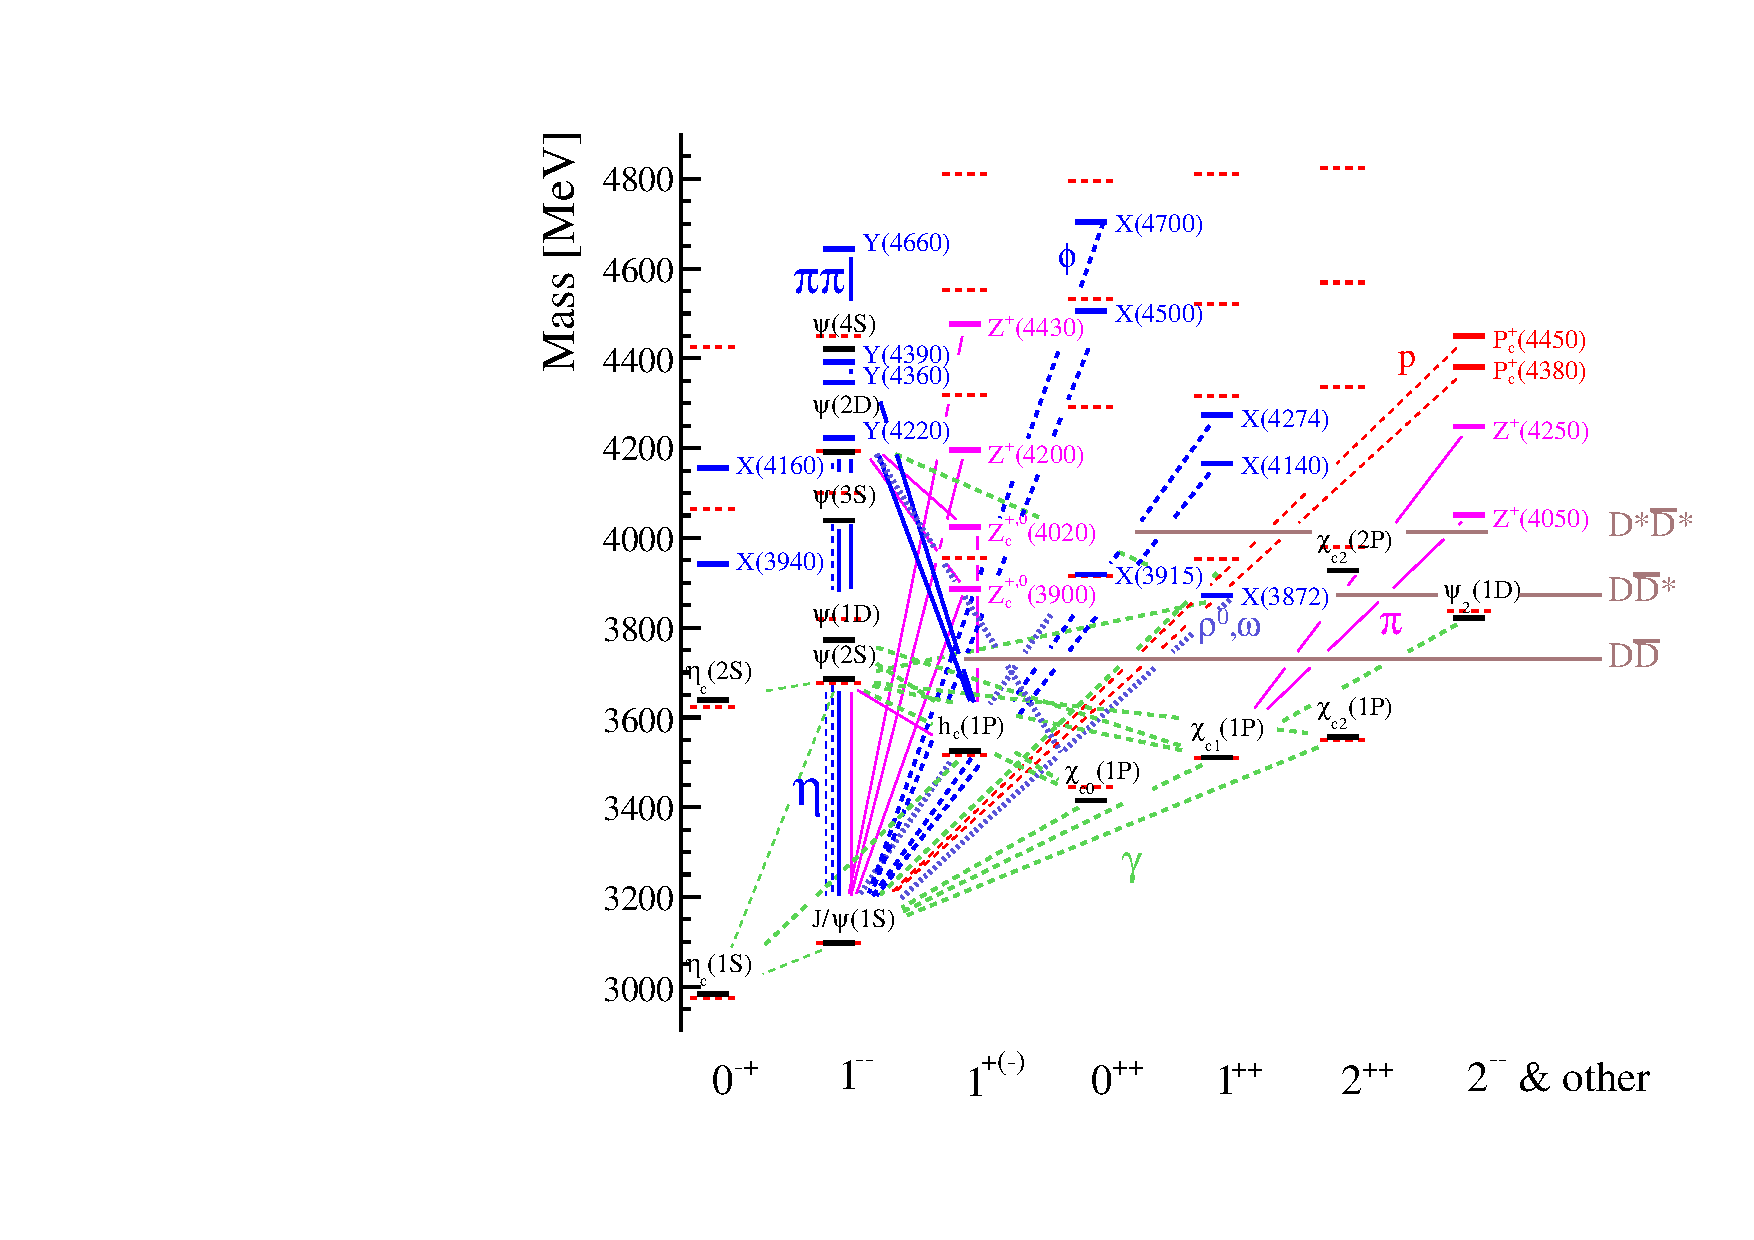
\includegraphics[width=15cm]{charmoniumExotic.pdf}
    \caption{The status of charmonium spectrum in August 2017. Red dashed lines represent theoretical predictions based on Godfrey-Isgur model with relativistic corrections to higher-excited states~\cite{gbs-model}. Black solid lines are experimentally measured energy levels. Here are also shown measured transitions. We are interested in radiative transitions which are represented by green dashed lines: thick for E1 and thin for M1. Source: Olsen, Skwarnicki, Zieminska~\cite{heavy-quark_pics}} \label{fig:charm-states}
\end{figure}

Regarding arguments for investigating charmonium. Charmonium is a two-particle system, the simplest possible system consisting of quarks. Constituent $c$-quarks possess huge mass ($\approx 1.27 GeV$) in comparison to $u$, $d$ and $s$ quarks ($\approx 0.1 GeV$). This allows us to apply non-relativistic phenomenological models for description of low-lying states. Moreover, the system is compact (we can estimate by order of magnitude $R \approx \alpha_a \cdot m_cS \approx 1 Fm$), so asymptotic freedom assumption is applicable as a boundary condition for the potentials.\cite{charm-slides}

Nevertheless, as one can see from the plot \cref{fig:charm-states}, even low-lying states like $\chi_c0(1P)$ have dramatic discrepancies with experiment. This gives a clue that there is something beyond Coulomb model even in non-relativistic description of charmonium states.

\paragraph{Multiquark states}
Beyond to some extent well known mesons and baryons there are also 4-quark states. They firstly were observed not so long time ago, in 2003 by Belle collaboration. There are two widely spread approaches have been described in literature~\cref{fig:charm-models}: molecular state~\cite{molecular-model} and tetraquark~\cite{tetraquark-model}.

\begin{figure}[H]
    \centering
    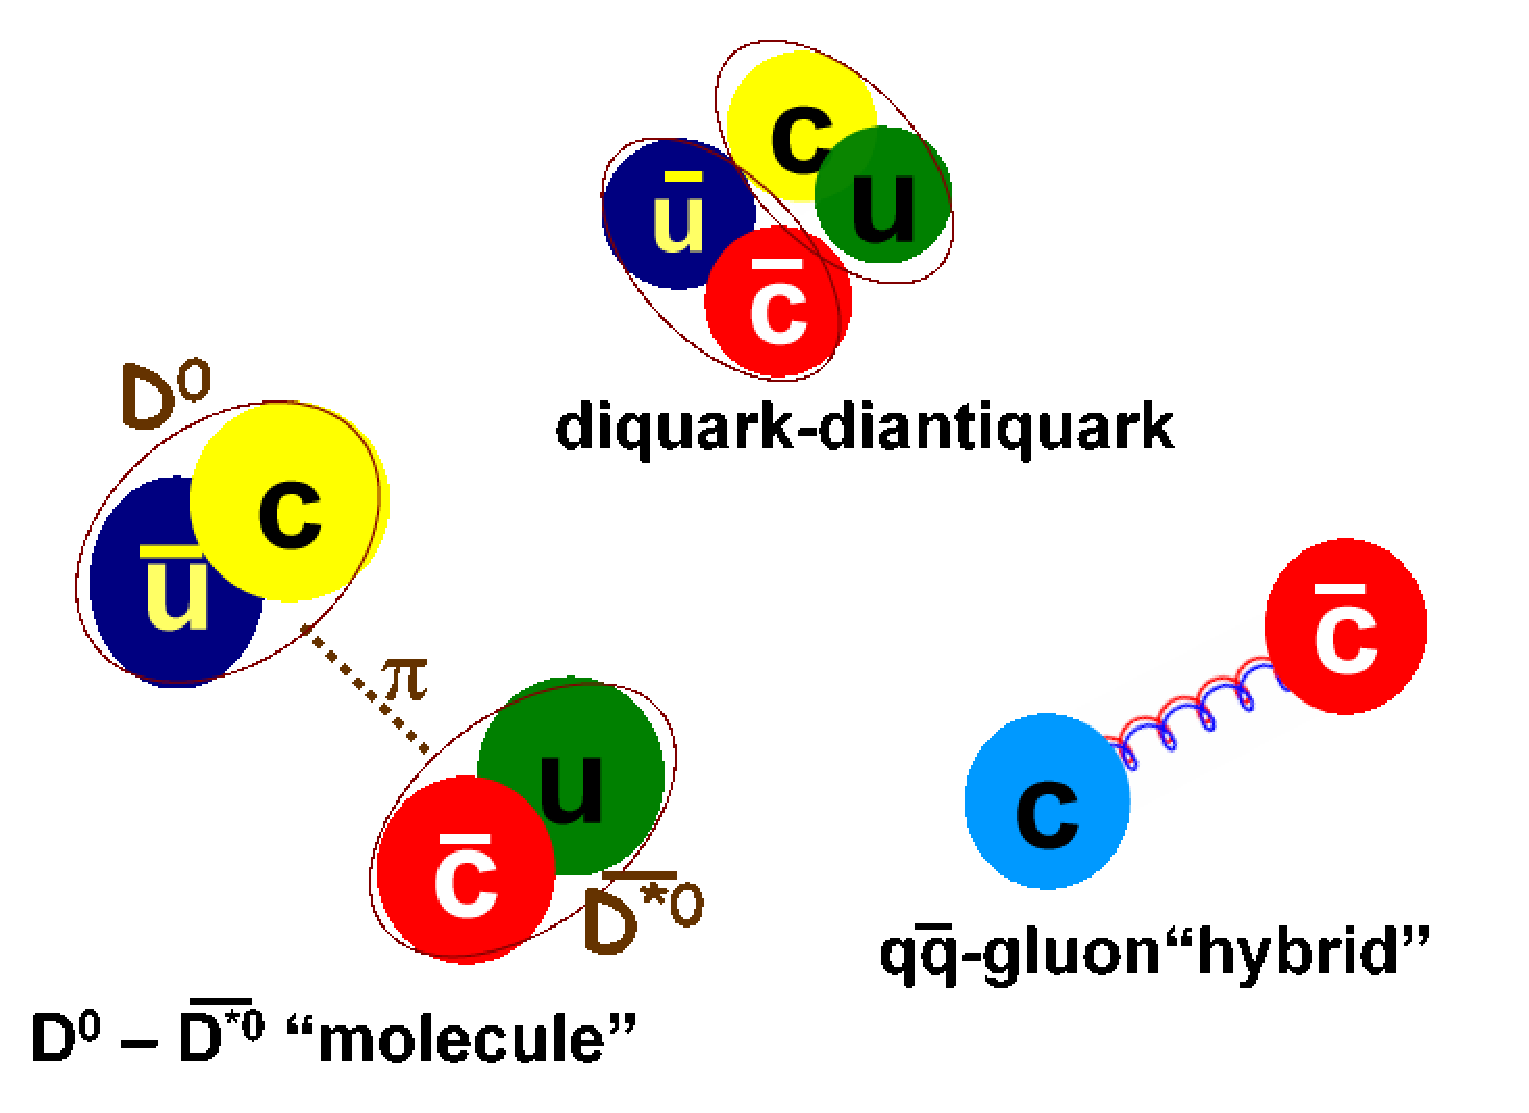
\includegraphics[width=12cm]{charm-models.eps}
    \caption{Multiquark models. left - molecular state, top - tetraquark, right - hybrid state\label{fig:charm-models}}
\end{figure}

Tetraquark state is modeled as an interaction of two pairs of quarks. Pairs don't carry integer charge, so can't be observed in a free state. Such a configuration assures tight-binding.

According to molecular model, quarks in 4-quark system are paired into meson-states which then interact with each other. They form a kind of a mesonic molecule. Our sumrules approach can find an application to or at least acquires some corrections from states with this kind of binding, because one of constituent mesons could appear to be charmonium state, and will contribute to sumrules.

The third model is not in the list of multiquark, but it is another way towards ``exotic'' states. The model named ``hybrid'', because apart of quarks it takes into account excited gluon mode, so it describes hybrid of quarks and gluons. Besides analytical calculations developed in this workflow~\cite{hybrid-th}, there are also motivating lattice works~\cite{hybrid-lattice1, hybrid-lattice2}. 

\paragraph{Experimental progress}
Plethora of new states has become accessible to experimentalists owing to B-factories --- high-luminocity $e^+ e^-$-colliders developed for testing $CP$-violation in Standard Model. They produce large number of $B\bar{B}$ coherent pairs. There are several ways to produce charmonium from such pairs excellently reviewed by Stephen Godfrey and Stephen Olsen in their paper ``The Exotic XYZ Charmonium-like Mesons''~\cite{godfrey-olsen}.

The dominant decay mechanism of a $B$ meson is through the $W$-boson with emission of a charm quark. A schematic diagram of the process is presented in the figure~\cref{fig:charmgen-bdecay}.

\begin{figure}[H]
    \centering
    \begin{subfigure}[b]{0.4\textwidth}
        \includegraphics[width=\textwidth]{charmgen-bdecay.pdf}
        \caption{direct $B$-decay} \label{fig:charmgen-bdecay}
    \end{subfigure}
    \begin{subfigure}[b]{0.4\textwidth}
        \includegraphics[width=\textwidth]{charmgen-isr.pdf}
        \caption{ISR} \label{fig:charmgen-isr}
    \end{subfigure}
    \caption{Production of charmonium}
\end{figure}

In case if $c$ and $\bar{c}$ quarks are produced close to each other, there is a probability for them to generate a bound state of charmonium. In such a process not all parity configurations are allowed. In the list of allowed ones are: $0^{-+}$, $1^{--}$, $1^{++}$. Thanks to this scheme Belle collaboration discovered $\eta^\prime_c$ meson in 2002.~\cite{bdecay-etacprime}

Another scheme is shown in~\cref{fig:charmgen-isr}. According to the diagram, charmonium is produced by photon, which is emitted due to annihilation of initial state electrons. For this reason, the process is named ``Initial State Radiation''(ISR). Center of mass energy of the radiated $\gamma$-ray should be $4000-5000\;MeV$, then production of charmonium $1^{--}$ will become possible. BaBar group uses ISR method to make measurement involving $J/\psi$ meson.~\cite{isr-jpsi}

\begin{figure}[H]
    \centering
    \begin{subfigure}[b]{0.4\textwidth}
        \includegraphics[width=\textwidth]{charmgen-assoc.pdf}
        \caption{Associated production} \label{fig:charmgen-assoc}
    \end{subfigure}
    \begin{subfigure}[b]{0.4\textwidth}
        \includegraphics[width=\textwidth]{charmgen-digamma.pdf}
        \caption{Double-$\gamma$ scheme} \label{fig:charmgen-digamma}
    \end{subfigure}
    \caption{Production of charmonium}
\end{figure}

Initial state radiation scheme can be extended to higher energies. According to observations of Belle group, when $J/\psi$ in final state has been observed then there is a high probability to find another charmonium state alongside~\cref{fig:charmgen-assoc}. Due to such a ``partnership'' this method got its name ``Associatied production''. Despite the fact that cross-section of such a process is very low, high luminosity of $B$-factories compensates  the shortage. Regarding parities, only $C=+$ is allowed. Experimentally only $0^{++}$ $\eta_c$ and $\eta_c^\prime$ have been observed, but $1^{++}$ and $2^{++}$ are not seen still.~\cite{assoc-prod}

Finally, we arrive to completely different production scheme ``Two photon scheme''~\cref{fig:charmgen-digamma}. $J^{PC}$ in that process allows $0^{-+}$, $0^{++}$, $2^{-+}$ and $2^{++}$. Thanks to this production scheme CLEO group has confirmed $\eta_c^\prime$ meson.~\cite{digamma}

\section{Superconvergent summation rule}
After the brief discussion of phenomenology and experimental facilities, let's have a look at the tool we are going to apply at the theoretical side of the work.

Originally,  the idea of sumrules comes from Gerasimov and Drell~\cite{gdh-g-orig} and independently Hearn~\cite{gdh-dh-orig} in application to forward Compton scattering. Well structured review on this topic has been provided by Klaus Halbing~\cite{gdh-helbing}. In 2010 a new application of the same scheme emerged. Marc Vanderhaeghen and Vladimir Pascalutsa applied GDH approach to Light-by-Light scattering process~\cite{lbl-sum1}. Firstly, it was developed for on-shell photons, but in 2012 together with Vladislav Pauk they published an article~\cite{lbl-sum2}, where sumrules emerge in LBL-scattering involving virtual photons~(\cref{fig:lbl-scatt}). 

\begin{align} \label{eq:lbl-scatt}
    \gamma^\star_1(\lambda_1, q_1) + \gamma^\star_2(\lambda_2, q_2) \rightarrow \gamma^\star_1(\lambda_1^\prime, q_1) + \gamma^\star_2(\lambda_2^\prime, q_2) 
\end{align}

\begin{figure}
    \centering
    \includegraphics[width=10cm]{lbl-scatt.pdf}
    \caption{Forward Light-by-Light scattering with virtual photons \label{fig:lbl-scatt}}
\end{figure}

First step of the derivation makes use of unitarity of the $S$-matrix and generates an optical theorem in case of forward scattering:

\begin{align}
    & S^\dag S = \Erm \\
    & S = \Erm + \ii T \\
    & T^\dag T = -\ii(T - T^\dag)
\end{align}

After inserting an operator identity at the lhs: $T^\dag T = \sum_{n} T^\dag \ket{n}\bra{n} T$ we arrive to the following expression:

\begin{align}
    & \sum_{n} \bra{out} T^\dag \ket{n}\bra{n} T \ket{in} = -\ii \left( \bra{out} T \ket{in} - \bra{out} T^\dag \bra{in} \right)
\end{align}

Let's recall that matrix element in QFT is actually a $T$-matrix element:

\begin{align}
    & \bra{out} T \ket{in} = \Mcal(in \rightarrow out) \qquad &\bra{out} T^\dag \ket{in} = \Mcal^\star(in \rightarrow out)
\end{align}

\begin{align}
        & \sum_{n} \Mcal(in \rightarrow n)  \Mcal(n \rightarrow out) = 2 \Im \Mcal(in \rightarrow out) \\
        & \int \lips{p} \abs{\Mcal(in \rightarrow \vec{p})}^2 = 2 \Im \Mcal(in \rightarrow in)
\end{align}

One should assume integration over all final momenta. Then, lhs can be expressed in the form of the total cross-section:

\begin{align}
    & 2 E_{c.m.} p_{c.m.} \sigma_{tot}(in \rightarrow \forall) =  \Im \Mcal(in \rightarrow in) \label{eq:optical-th}
\end{align}

Another ingredient of sumrules ``cocktail'' is the analyticity of amplitudes. We assume that $\Mcal$ doesn't contain any poles except physical ones, which correspond to bound states of the system. Formally, this statement can be expressed by Cauchy's theorem. We use Schwartz principle to conduct analytical continuation of the amplitude. See details in appendix~\cref{sec:app:alyt-ampl}. As a result we obtain:

\begin{align}
    & \Mcal(s) = \frac{1}{\pi} \fint \frac{\Im \Mcal(s^\prime + \ii \epsilon)}{s^\prime - s} \dd{s^\prime} \\
    & \Re \Mcal(s + \ii \epsilon) = \frac{1}{\pi} \fint \frac{\Im \Mcal(s^\prime + \ii \epsilon)}{s^\prime - s} \dd{s^\prime} \label{eq:disp-rel-gen}
\end{align}

In case of the forward scattering matrix element acquires a beautiful parity structure. It will help us to simplify the dispersion relation above. Parity relations involve helicities of initial and final photons, that is why working in terms of amplitudes with defined helicities is convenient.

We denote $\Mcal_{\lambda^\prime_1 \lambda^\prime_2 \lambda_1 \lambda_2}$ an amplitude, where the first photon ($\gamma_1$) has helicity $\lambda_1$ in the initial state and $\lambda_1^\prime$ in the final state. The same holds for the second photon $\gamma_2$. As photons are virtual, possible values for $\lambda$ include $\lambda=0$ besides usual $\lambda=\pm1$.

In this terms we can express symmetry under parity and time reversion:

\begin{align}
    & \mathcal{P}:\quad \Mcal_{\lambda_1^\prime \lambda_2^\prime \lambda_1 \lambda_2} = \Mcal_{-\lambda_1^\prime -\lambda_2^\prime -\lambda_1 -\lambda_2} \\
    & \mathcal{T}:\quad \Mcal_{\lambda_1^\prime \lambda_2^\prime \lambda_1 \lambda_2} = \Mcal_{\lambda_1 \lambda_2 \lambda_1^\prime \lambda_2^\prime}
\end{align}

Taking into account above symmetries, there are only eight independent amplitudes left. They can be combined into even and odd under parity.

\begin{align}
    &\text{Even:}~f^{(+)}(\nu) = f^{(+)}(-\nu) && \\ \nonumber
    &(\Mcal_{++,++}-\Mcal_{+-,+-}) &\Mcal_{++,--}\qquad &\Mcal_{00,00}\\
    &\Mcal_{+0,+0} &\Mcal_{0+,0+}\qquad &(\Mcal_{++,00} + \Mcal_{0+,-0})\\
    &\text{Odd:}~f^{(-)}(\nu) = -f^{(-)}(-\nu) && \\ \nonumber
    &(\Mcal_{++,++} - \Mcal_{+-,+-}) & &(\Mcal_{++,00} - \Mcal_{0+,-0})
\end{align}

To make use of crossing symmetry, it is convenient to parametrize amplitudes in terms of variable $\nu = \frac{1}{2} (s - u) = q_1 q_2$, which only changes sign under crossing transformation of one of the photons.

For the sake of generality we'll use $f^{(+)}$ and $f^{(-)}$ for even and odd amplitudes correspondingly. Then, it is possible to simplify dispersion relation in \cref{eq:disp-rel-gen}:

\begin{align}
    \Re f^{(+)}(\nu + \ii \epsilon) = \frac{2}{\pi} \int_{\nu_0}^{\infty} \dd{\nu^\prime} \frac{\nu^\prime}{\nu^{\prime 2} - \nu^2} \Im f^{(+)}(\nu^\prime + \ii \epsilon) \\
    \Re f^{(-)}(\nu + \ii \epsilon) = \frac{2\nu}{\pi} \int_{\nu_0}^{\infty} \dd{\nu^\prime} \frac{1}{\nu^{\prime 2} - \nu^2} \Im f^{(-)}(\nu^\prime + \ii \epsilon)
\end{align}

Where we used crossing symmetry relation to map negative half-plane onto positive:

\begin{align}
    & \text{Crossing:}\quad \Mcal_{\lambda_1^\prime \lambda_2^\prime \lambda_1 \lambda_2}(\nu) = \Mcal_{\lambda_1^\prime -\lambda_2 \lambda_1 -\lambda_2^\prime}(-\nu)
\end{align}


We introduced $\nu_0$, a threshold at which final particle state becomes forbidden.

At this point we find out eight relations connecting real part of helicity amplitudes to their imaginary part, and according to the optical theorem~\cref{eq:optical-th} to corresponding helicity cross-sections. We'll focus on the odd amplitude $(\Mcal_{++,--} - \Mcal_{+-,+-})$, because there exists low energy theorem, an estimation for the value of $\frac{f^{(-)}(\nu)}{\nu}$ in the limit of $\nu \rightarrow \nu_0$. By analogy to GDH sumrule for the Compton scattering based on perturbation theory, value of the latter expression can be expressed in terms of anomalous magnetic moment ($a$) and mass ($m$) of the vector meson:

\begin{align}
    \frac{f^{(-)}(\nu)}{\nu} \rightarrow 16 \pi \frac{\alpha_{EM}}{m^2} a^2 \approx 70 nb \text{\quad \textit{for charmonium}}
\end{align}

This is quite small number when comparing to magnitudes of partial decay width for transitions contributing into sumrule. We assume it negligibly small and, finally, arrive to the superconvergent relation:

\begin{center} \fbox{
    \parbox{10cm}{
        \centering
        \begin{equation} \label{eq:sumrule-sigma}
            \large
            \int_{s_0}^\infty \frac{\sigma_2(s) - \sigma_0(s)}{s - m^2} \dd{s} = 0
        \end{equation}
    }
} \end{center}

\paragraph{Charmonium in the final state}
When we are looking at radiative transitions between charmonium bound states, the superconvergent relation~\cref{eq:sumrule-sigma} simplifies a lot. In the transition we actually have a process $2 \rightarrow 1$, which naturally can be expressed in terms of decay width $1 \rightarrow 2$. This unsual kind of cross-section has a remarkable property. It is zero as a function of energy almost everywhere except regions near bound states, where cross-section acquires sharp peaks. Relation between cross-section and decay width is easy to derive in center of mass frame (see the full derivation in Appendix~\cref{eq:app:crsc-dw}):

\begin{align} \label{eq:crsc-dw}
    \sigma = \frac{16 \pi^2 m_f^3}{(m_f^2 - m_i^2)^2} (2J_f + 1) \Gamma \delta(s - m_f^2)
\end{align}

The expression is derived for specific final state, and one can notice a delta-function which expresses a sharp behavior near the bound state mass. Let's substitute this result into~\cref{eq:sumrule-sigma}, summing up over all possible final states:

\begin{align}
    \sum_{m_f} \frac{16 \pi^2 m_f^3}{(m_f^2 - m_i^2)^3} (2J_f+1) \left\{ \Gamma\left[m_f \rightarrow (\Lambda = +-)\right] - \Gamma\left[m_f \rightarrow (\Lambda = ++)\right] \right\} = 0
\end{align}

Here $m_f \rightarrow (\Lambda = ++)$ corresponds to the process, where photon and vector meson have helicities $+$, and the bound state which emerge from unitarity has mass $m_f$ and helicity $0$, because total helicity is defined with a minus sign: $\Lambda = \lambda_\gamma - \lambda_i$. From the experimental point of view $\Gamma\left[m_f \rightarrow (\Lambda=0)\right] = \Gamma\left[m_f \rightarrow (\Lambda = ++)\right] + \Gamma\left[m_f \rightarrow (\Lambda = --)\right]$ makes more sense. The same holds for $\Lambda=2$. Taking into account that both terms are equal due to symmetry under parity, the expression above acquires a factor $\frac{1}{2}$:


\begin{align} \label{eq:sumrule-dw-nosub}
    \sum_{m_f} \frac{8 \pi^2 m_f^3}{(m_f^2 - m_i^2)^3} (2J_f+1) \left\{\Gamma\left[m_f \rightarrow (\Lambda = 2)\right] - \Gamma\left[m_f \rightarrow (\Lambda = 0)\right] \right\} = 0
\end{align}

During the derivation we assumed all final states being heavier than vector meson. But even for $J/\psi$ there exists charmonium state which lies underneath ($\eta_c$). In that case, we can keep notation meaning the decay happening in the reveresed direction: $\gamma \eta_c \leftarrow J/\psi$. Cross-section $\gamma + J/\psi \rightarrow \eta_c$ can be mapped to the corresponding decay width using parity, time reversal and crossing symmetry (see Appendix~\cref{eq:app:crsc-dw-subthr}). What is remarkable in such a mapping, it translates $\sigma(\Lambda=++)$ into $\Gamma(\Lambda=+-)$, i.e. swaps the helicity of photon and switches total helicity from $0$ into $2$ and vice versa. As a result, the ``subthreshold pole'' will contribute with inversed sign when written in terms of decay widths. Let's append subthreshold contributions into~\cref{eq:sumrule-dw-nosub}:

\begin{align} \label{eq:sumrule-dw}
    &-\sum_{m_f < m_i} \frac{8 \pi^2 m_i^3}{(m_i^2 - m_f^2)^3} (2J_i+1) \left\{\Gamma\left[m_i \rightarrow (\Lambda = 2)\right] - \Gamma\left[m_i \rightarrow (\Lambda = 0)\right] \right\} + \nonumber \\
    &+ \sum_{m_f > m_i} \frac{8 \pi^2 m_f^3}{(m_f^2 - m_i^2)^3} (2J_f+1) \left\{\Gamma\left[m_f \rightarrow (\Lambda = 2)\right] - \Gamma\left[(\Lambda = 0) \rightarrow m_f\right] \right\} = 0
\end{align}

Notice that all bound states of charmonium contribute to the sum, so having information about radiative transitions at low energy levels we have direct estimate for contributions of the transitions from high-energy states. Another important remark is that to~\ref{eq:sumrule-dw} contribute decay widths of different helicities, at the same time at experiment people usually measure total decay widths. As we would like to use experimental data, we need to develop some way of distinguishing between helicity contributions. Formally we can introduce translating coefficients corresponding to relative contribution of each helicity to the total radiative decay width:

\begin{align}
    r^{(0)} = \frac{\Gamma\left[m_f \leftrightarrow (\Lambda=0)\right]}{\Gamma_{tot}} \\
    r^{(2)} = \frac{\Gamma\left[m_f \leftrightarrow (\Lambda=2)\right]}{\Gamma_{tot}}
\end{align}

These coefficients are not universal but depend on the states taking part in transition. Process of calculation of the coefficients consists of several steps. First of all we are going to solve for eigenvalues non-relativistic Shrodinger equation with potential given by non-relativistic quark model. Eigenvalues correspond to masses of charmonium bound states. Then we can use eigenvalues to get eigenfunctions, i.e. wave functions of corresponding bound states. Finally, having wave functions, we can apply Pauli equation to model electromagnetic interaction between quarks in a bound state, in this way we'll be able to estimate decay widths of radiative transitions.

\section{Non-relativistic quark model}
According to the plan, we are in need of some model to reproduce masses and wave functions of charmonium. For the low-energy region non-relativistic quark model does well in reproducing experimental results~\cite{deng-charm, deng-bot}. Here we are going to introduce the model potential based on phenomenological considerations introducing empirical fitting parameters, but at the same time we are referring to the sources where the model has been obtained from non-relativistic limit of QCD perturbation theory~\cite{nrqm-perturb}. Thus physical meaning of the parameters to some extent can be traced.

Starting from two-quark Shrodinger equation we can pass to the center of mass frame. We denote by $\vec{r}$ a vector pointing from quark to anti-quark. The problem is spherically symmetric, so we can decouple angular dependency into spherical harmonic $Y_{Lm}$. We consider $\hbar = c = 1$ convention:

\begin{align}
    &\left[ -\frac{1}{2 \mu_R} \Delta_{\vec{r}} + V(\abs{\vec{r}}) \right] \psi(\vec{r}) = E_{bound} \psi(\vec{r}) \\
    &\dv[2]{u(r)}{r} + 2 \mu_R \left[ E_{bound} - V(r) - \frac{L(L+1)}{2 \mu_R r^2} \right] u(r) = 0 \\
    &\abs{\vec{r}} = r ,\quad \psi(\vec{r}) = \frac{u(r)}{r} Y_{Lm}(\Omega) \\
    &V(r) = V_V(r) +V_S(r) + V_{SL}(r) + V_{SS}(r) + V_T(r)
\end{align}

This is a general form of the equation for charmonium spectrum. Let's step through each term contributing to the potential.

\begin{align} \label{eq:nrqm-vv}
    V_V(r) = -\frac{4}{3} \frac{\alpha_S}{r}
\end{align}

Coulomb-like interaction between quark and anti-quark(\cref{eq:nrqm-vv}) comes from the one-gluon exchange process. Asymptotic freedom can be included in running strong coupling $\alpha_S$, but for the sake of simplicity we leave it as a constant parameter.

Another distinctive feature of QCD, confinement, is encoded into the growing behavior of the potential when quarks move away from each other. A kind of gluon string tension streched between quark and anti-quark. There are two models presented in \cref{eq:nrqm-vs}: linear and screened. The latter, in addition to the string tension tries to model a process when distantly placed quarks acquire screening between each other by pulling new quark-antiquark pairs from vacuum. Parameter $\mu$ is related to the distance at which birth of new pairs becomes possible, and $b$ describes tention force in linear approximation.

\begin{align} \label{eq:nrqm-vs}
    V_S(r) = \left[ \begin{matrix*}[l]
                    &\text{Linear:}\quad br \\
                    &\text{Screened:}\quad \frac{b}{\mu} (1 - \exp^{-\mu r})
              \end{matrix*} \right.
\end{align}

Spin-orbit coupling(\cref{eq:nrqm-sl}) is well-known in two-body problem. It appears as an evidence of non-commutativity of Lorentz transformations. At the classical level it emerges as ``Thomas precession''~\cite{thomas}

\begin{align} \label{eq:nrqm-sl}
    V_{SL}(r) = \frac{1}{2 m_c^2 r} \left( 3 \dv{V_V}{r} - \dv{V_S}{r} \right) \vec{L} \cdot \vec{S}
\end{align}

Spin-spin interaction (\cref{eq:nrqm-ss}) is based on perturbative expansion of $T$-matrix by $\frac{v}{c}$, and has a contact nature. For numerical purposes we follow~\cite{gbs-model} and smear the delta-function at the scales of order $\frac{1}{\sigma} \propto \frac{1}{m_c}$:

\begin{align} \label{eq:nrqm-ss}
    V_{SS}(r) = \frac{32 \pi \alpha_S}{9 m_c^2} \tilde{\delta}_\sigma(r) \vec{S}_c \cdot \vec{S}_{\bar{c}},\quad \tilde{\delta}_\sigma(r) = \left(\frac{\sigma}{\sqrt{\pi}}\right)^3 \ee^{-\sigma^2 r^2}
\end{align}

Tensor term(\cref{eq:nrqm-t}) is another product of perturbative expansion. It is important to mention that this term introduces a hyperfine splitting of levels over total angluar momentum projects.

\begin{align} \label{eq:nrqm-t}
    &V_T(r) = \frac{1}{12 m_c^2} \left( \frac{1}{r} \dv{V_V}{r} - \dv[2]{V_V}{r} \right) \vec{H}_T \\
    &\vec{H}_T = 6\frac{(\vec{S} \cdot \vec{r})^2}{r^2} - 2\vec{S}^2
\end{align}

To simplify computations we decieded to omit hyperfine splitting by averaging tensor term over total angular momentum projections. As a result we obtain the following result(for derivation see the appendix (\cref{sec:app:tensor-term}). Round brackets here represent $6j$ symbol.

\begin{align}
    &V_T(r) = \frac{1}{12 m_c^2} \left( \frac{1}{r} \dv{V_V}{r} - \dv[2]{V_V}{r} \right) \left<\vec{H}_T\right> \\
    &\left<\vec{H}_T\right> = 2 (-1)^{L+S-J+1} \sqrt{\frac{L(L+1)(2L+1)}{(2L-1)(2L+3)}} \times \nonumber \\
    &\qquad \times \sqrt{S(S+1)(2S+1)(2S+3)(2S-1)} \left( \begin{matrix}
                                                L & J & S \\
                                                S & 2 & L
                                              \end{matrix} \right)
\end{align}

Finally, having binding energies and wavefunctions of charmonium states obtained we can apply Pauli equation to the quark-antiquark system to describe raditive transitions. In the next chapter we discuss this approach briefly reminding apparatus of the multipole decomposition which comes in handy for analytical calculations.

\section{Electromagnetic transitions between charmonium states}
We would like to start this chapter by reminding the main goal --- computation of $r^{(0,2)}$ coefficients for charmonium system. The general expression for decay width has been presented above, when we connected cross-section $2 \rightarrow 1$ with it. In assumption that all states follow covariant normalization, expression had the following form:

\begin{align}
    &\Gamma = \frac{m_f^2 - m_i^2}{16 \pi m_f^3} \frac{1}{2J_f + 1} \sum_{\lambda_f} \abs{\Mcal_{\lambda_f, \lambda_i \lambda_\gamma}}^2
\end{align}

For our purposes it will be convenient to use quantum mechanical normalization for initial and final charmonium states(see ~\cref{par:app:dw-nr}). We also pulled out electron charge from $H_{int}$ to combine it into the coupling constant $\alpha = \frac{e^2}{4 \pi}$: 

\begin{align}
    &\Gamma = \alpha \frac{m_f^4 - m_i^4}{2 m_f^3} \frac{1}{2J_f + 1} \sum_{\lambda_f} \abs{\Mcal_{\lambda_f, \lambda_i \lambda_\gamma}}^2 \label{eq:dw-nr} \\
    &\Mcal_{\lambda_f, \lambda_i \lambda_\gamma} = \int \dd{r} \psi_f^\star(r) \bra{J_f j_f L_f S_f} H_{int}^{\lambda_\gamma} \ket{J_i j_i L_i S_i} \psi_i(r) \label{eq:mel-nr}
\end{align}

We assume electromagnetic field being hardcoded into $H_{int}$, so instead of creation/annihilation operators hamiltonian acquires photon helicity index. Regarding helicities of initial and final state, they are encoded into angular momentum projections. In the center of mass frame decay products both have outgoing momenta, thus by orienting quantization axis along photon momentum, angular momenta can be translated into helicities with the following rule:

\begin{align}
    j_f \leftrightarrow -\lambda_f \qquad j_i \leftrightarrow \lambda_i
\end{align}

Then angular momentum conservation can be reformulated in terms of helicities. This confirm that our matching respects notion of ``total helicity'' used in previous chapters.

\begin{align}
    j_i = j_f + \lambda_\gamma \leftrightarrow \lambda_i = \lambda_\gamma - \lambda_f
\end{align}

In expressions~\cref{eq:dw-nr,eq:mel-nr} all quantities except $H_{int}$ we already know. The latter we'll derive based on Pauli equation for quark-antiquark system. Notice that when free of charges EM field in Coulomb gauge ($\nabla\cdot\vec{A} = 0$) respects $A_0 = 0$ as well (see lectures of David Tong for details~\cite{tong-qed}). We also ignore non-linearities, i.e. self-interaction of photons:

\begin{align}
    &\left[\frac{1}{2m_q} \left( \vec{\sigma}_q \cdot [\vec{p}_q - e_q \vec{A}(\vec{r}_q)] \right)^2 + \frac{1}{2m_{\bar{q}}} \left( \vec{\sigma}_{\bar{q}} \cdot [\vec{p}_{\bar{q}} - e_{\bar{q}} \vec{A}(\vec{r}_{\bar{q}})] \right)^2 + V(r) \right] \psi = \ii \pdv{t} \psi \\
    &\left[H_0 + H_{int} \right] \psi= \ii \pdv{t} \psi \\
    &H_{int} = \sum_{i = q, \bar{q}} -\frac{e_i}{m_i} \vec{A}(\vec{r}_i) \vec{p}_i - \frac{e_i}{2 m_i} \vec{\sigma} \cdot \rot_i \vec{A}(\vec{r}_i)
\end{align}

Here $V$ is a potential for non-relativistic quark model, $H_0$ includes kinetic terms and $V$ and describes bound states of charmonium in vacuum. Finally $H_{int}$ -- part responsible for the interaction of charmonium with EM field.

Taking into account that we have a quark-antiquark system, charges of the particles differ only by sign and we can rewrite $H_{int}$ in the center of mass frame grouping similar terms:

\begin{align} \label{eq:hint-nomult}
    &H_{int} = -\frac{e}{2 \mu_R} \vec{p} \left[ \vec{A}(\frac{\vec{r}}{2}) + \vec{A}(\frac{-\vec{r}}{2}) \right]-\frac{\lambda_\gamma k e}{4 \mu_R}\left[ \vec{\sigma}_q \vec{A}(\frac{\vec{r}}{2}) - \vec{\sigma}_{\bar{q}} \vec{A}(\frac{-\vec{r}}{2}) \right]
\end{align}

Notice $k \lambda_\gamma$ emerged instead of $\rot$. As far as photons are represented by plane waves, it's easy to check the following statement. Moreover, it doesn't depend on whether photon was emitted or absorbed:

\begin{align}
    &\rot_i \vec{A_{\vec{k}, \lambda_\gamma}(\vec{r}_i)} = \lambda_\gamma k \vec{A}_{\vec{k}, \lambda_\gamma}(\vec{r}_i)
\end{align}

The~\cref{eq:hint-nomult} can be shorten by half making use of parity. For further analysis it will be convenient to expand EM field into multipole series. Each multipole transforms in a defined way under parity, so $H_{int}$ acquires simpler form:

\begin{align} \label{hint-mult-nobrak}
    &H_{int}^{EJ} = \left[ -(E_f - E_i) \ii e \vec{r} \delta_{2 \nmid J} - \frac{\lambda_\gamma k e}{2 \mu_R} \delta_{2 \mid S_i + S_f + J} \vec{\sigma}_q \right] \vec{A}^{EJ}(\frac{\vec{r}}{2}) \\
    &H_{int}^{MJ} = \left[ - \frac{\lambda_\gamma k e}{2 \mu_R} \delta_{2 \nmid S_i + S_f + J} \vec{\sigma}_q \right] \vec{A}^{MJ}(\frac{\vec{r}}{2}) 
\end{align}

Where multipoles are expressed in terms of vector spherical harmonics $\vec{Y}^\lambda_{J, l}(\Omega)$. Further we omit argument $\Omega$ because after we applied Wigner rotation to decaying state the only angle which takes place here could be one between $\vec{k}$ and $\vec{r}$:

\begin{align}
    &\vec{A}^{EJ}(\frac{\vec{r}}{2}) = \sqrt{2\pi} (-\ii)^{J+1} \left[ \sqrt{\frac{J+1}{2J+1}} j_{J-1}(\frac{kr}{2}) \vec{Y}^{-\lambda_\gamma}_{J-1, J} - \sqrt{\frac{J}{2J+1}} j_{J+1}(\frac{kr}{2}) \vec{Y}^{-\lambda_\gamma}_{J+1, J} \right] \\
    &\vec{A}^{MJ}(\frac{\vec{r}}{2}) = -\sqrt{2\pi} (-\ii)^J \sqrt{2J+1} \lambda_\gamma j_J(k r) \vec{Y}^{-\lambda_\gamma}_{J,J}
\end{align}

Assuming $H_{int}$ is under brackets $\bra{J_f j_f L_f S_f} H_{int} \ket{J_i j_i L_i S_i}$  we introduce $Q$ and $C$ symbols carrying all information about angular structure of the process:

\begin{align}
    &\sqrt{2L+1} C^\lambda_{L, J} = \bra{J_f j_j L_f S_f} \vec{\sigma}_q \vec{Y}^{\lambda}_{L, J} \ket{J_i j_i L_i S_i} \\
    &r Q^{\lambda}_{L, J} = \bra{J_f j_j L_f S_f} \vec{r} \vec{Y}^{\lambda}_{L, J} \ket{J_i j_i L_i S_i} = r \sqrt{2L+1} \braket{L010}{J0} Q^\lambda_J
\end{align}

In this terms, $\bra{J_f j_f L_f S_f} H_{int} \ket{J_i j_i L_i S_i}$ acquires the following form, which we'll directly use in our numerical computations (for complete derivation see~\cref{sec:app:hint-multipole}):

\begin{align}
    \begin{split}
        &H_{int}^{EJ} = -\sqrt{2\pi} (- \mathrm{i})^{J+1} \left[ 2 \mathrm{i} e (E_f-E_i) \delta_{2 \nmid J} (2J+1) \sqrt{J(J+1)} \frac{Q_{J}^{- \lambda}}{k} j_{J}(\frac{kr}{2}) + \right.\\
        &\qquad +  \frac{\lambda k e}{2 \mu} \delta_{2 \mid S_i + S_f + J} \left(  \sqrt{(J+1)(2J-1)} j_{J-1}(\frac{kr}{2}) C_{J-1, J}^{- \lambda} -\right. \\
        &\qquad\qquad\left.\left.- \sqrt{J(2J+3)} j_{J+1}(\frac{kr}{2}) C_{J+1, J}^{- \lambda} \right) \right]
    \end{split} \\
    &H_{int}^{MJ} = \sqrt{2\pi} (- \mathrm{i})^{J} (2J+1) j_J(\frac{kr}{2}) \frac{k e}{2 \mu} \delta_{2 \nmid S_i + S_f +J} C_{J, J}^{- \lambda}
\end{align}
